\chapter{Analysis Optimization}\label{sec:analysis_optimization}

Upon identifying objects that represent the final state of the physical process under investigation, a variable must be constructed from the event properties sensitive to the outcomes of a hypothesis test, typically with signal to background separation capabilities. Often, this variable takes the form of a kinematic variable, such as the invariant mass of the Higgs pair system ($m_\text{HH}$) from this analysis.

As elaborated in chapter \ref{sec:statistics}, the underlying statistical test employs frequentist principles, with histograms derived from this variable serving as inputs to these tests. Throughout the development of this variable, various optimizations typically aim to maximize the signal-to-background ratio, which acts as a proxy for the statistical test's expressivity.

Given the purpose of this variable to separate signal from background, it is well-suited for analysis with a \ac{ml} model. While such models have gained widespread usage in particle physics \citep{albertsson2019machine,shlomi2020graph,feickert2021living,Schwartz2021Modern}, their effectiveness is limited when they are only optimized for signal-to-background discrimination. This is because their training does not usually consider broader goals like assessing discovery significance or establishing confidence levels.

The signal-to-background ratio or the efficacy of a \ac{ml} model in separating events correlates to some extent with the performance of the statistical test. However, this relationship often remains suboptimal because uncertainties, which can significantly influence the outcome of hypothesis tests, are not typically considered during the training phase of \ac{ml} models.

To address these challenges, \textit{\acf{neos}} \citep{Simpson_2023} offers a promising solution. This approach integrates the statistical model and its uncertainties into the \ac{ml} model's training process, aligning it more closely with the primary goal of determining whether a new process exists. This chapter introduces machine learning concepts and elaborates on the \textit{\ac{neos}} methodology and its implementation in this analysis with the \ac{tomatos} training framework.


\section{Machine Learning}
\ac{ml} refers to algorithms that enable computers to learn from data and make predictions for specific tasks without being explicitly programmed for each task \citep{kubat2021introduction}. A notable subset of \ac{ml} models are \acp{ann}, which are inspired by the structure and function of the human brain. The fundamental units of \acp{ann} are nodes, or neurons, which are interconnected to other neurons. When these neurons are organized in consecutive layers with an initial input layer and a desired output layer, as shown in figure \ref{fig:ann} they are referred to as deep feed-forward \acp{nn}.
\begin{figure}
    \centering
    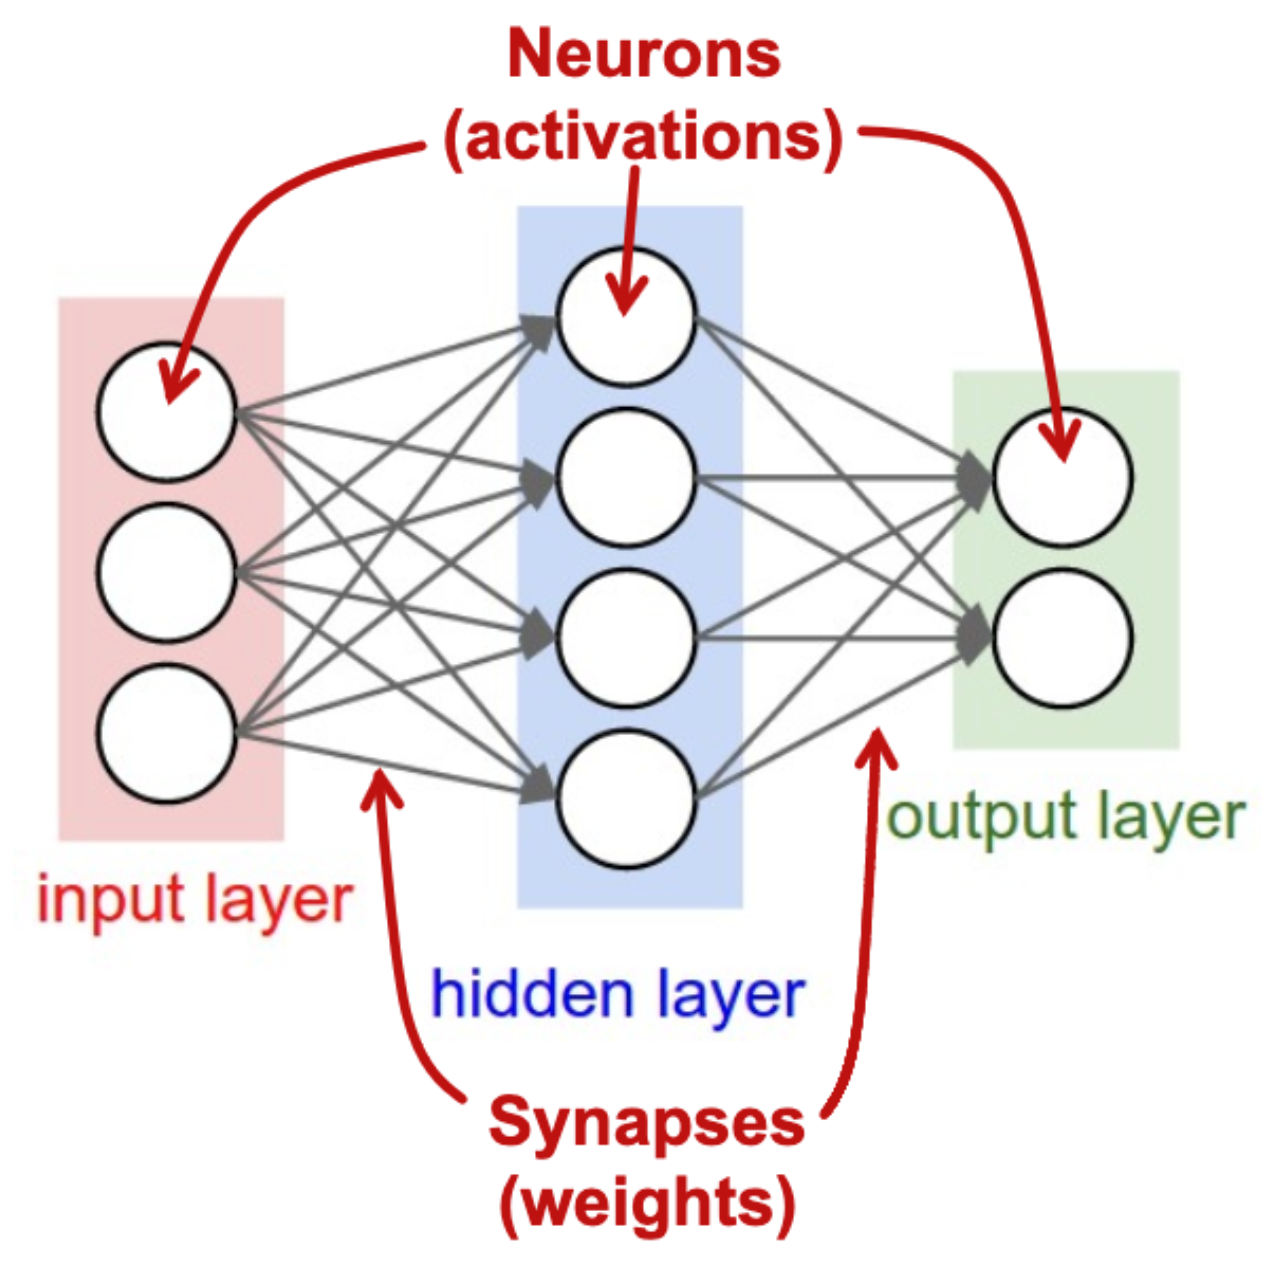
\includegraphics[width=0.4\textwidth]{ann}
    \caption[]{Structure of artificial feed-forward neural networks. Adopted from \citep{8114708}.}
    \label{fig:ann}
\end{figure}
In these networks, signals are transmitted between neurons via weighted connections denoted as $w_i$. The inputs to a neuron are summed, and each neuron has an additional bias or threshold term. This cumulative input is transformed by an activation function into an output signal:
\begin{equation}
    n_j=f_\text{activation} \left( \sum_{i\in \text{inputs}} w_i + n_j^\text{bias}\right).
\end{equation}
Typical activation functions include the Rectified Linear Unit (ReLU), defined as $f_\text{activation}=\max(0,x)$ and the sigmoid function, defined as  $f_\text{activation}=1/(1+e^{-x})$ which are illustrated in figure \ref{fig:activation_fun}.
\begin{figure}
    \centering
    \subfigure[]{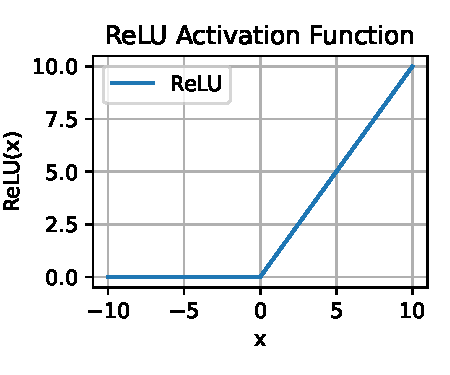
\includegraphics[width=.47\textwidth]{relu_activation_function}}
    \subfigure[]{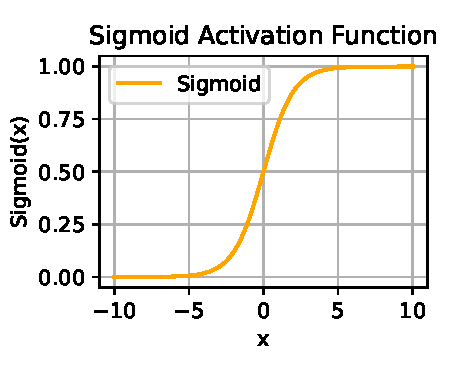
\includegraphics[width=.47\textwidth]{sigmoid_activation_function}}
    \caption[]{(a) Rectified Linear Unit and (b) Sigmoid activation functions.}
    \label{fig:activation_fun}
\end{figure}
The parameters $\bm{\varphi}$ of the \ac{nn} include the weights and bias terms of the neurons and learning occurs by adjusting these. \acp{ann} can be designed in various architectures and depths depending on the specific task.

Training \acp{nn} typically involves the back-propagation algorithm, which aims to minimize a cost  function $C(\bm{\varphi})$. This function measures the deviation of a given input from a desired output as a function of the model parameters $\bm{\varphi}$. For binary classification tasks, where outputs range continuously from 0 to 1 (with e.g. 1 indicating signal and 0 indicating background), the \ac{bce} cost function is commonly used:
\begin{equation}\label{eq:bce}
    C = -\frac{1}{N} \sum_{i=1}^{N} \left[ y_i \log(p_i) + (1 - y_i) \log(1 - p_i) \right],
\end{equation}
where $N$ is the total number of training examples, $y_i$ represents the true label and $p_i$ is the predicted value by the \ac{nn} for the $i$-th training example.

The minimum of this cost function can be found stepwise via gradient descent. Here, the update to the model parameters is guided by the negative of the gradient of the cost function, scaled by a learning rate $\gamma$
\begin{equation}
    \bm{\varphi}_{n+1} = \bm{\varphi}_n-\gamma\nabla C(\bm{\varphi}_n),
    \label{eq:grad_descent}
\end{equation}
such that moving against the gradient a monotonic decreasing series is formed $C(\bm{\varphi}_n )\ge C(\bm{\varphi}_{n+1})$ converging to a minimum of $C(\bm{\varphi})$. In three dimensions this is analogues to a mountaineer searching for the valley by going in the direction of the steepest descent with a stepsize proportional to $\gamma$.




\section{NEOS}
The core innovation of \textit{\ac{neos}} lies in integrating the hypothesis testing procedure into the training process of the \ac{nn}. Rather than employing a \ac{bce} cost function from equation \ref{eq:bce} focused solely on distinguishing between signal and background, the $\mathrm{CL}s$ value, detailed in Chapter \ref{sec:statistics}, is adopted as the quantity for minimization. As depicted in Figure \ref{fig:neos}, this approach effectively results in a mathematical concatenation of the individual steps within the typical analysis chain.

\begin{figure}
    \centering
    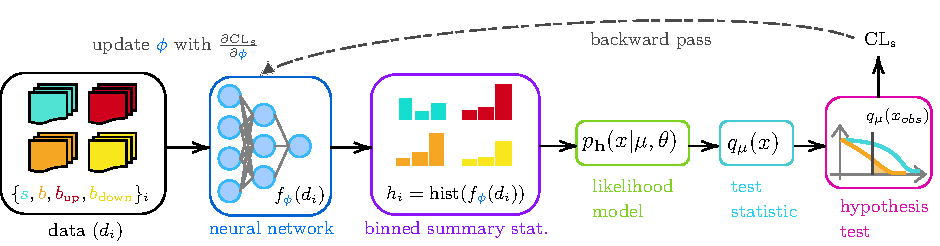
\includegraphics[width=1\textwidth]{neos}
    \caption[]{Typical particle physics analysis chain. For \ac{neos} the $\text{CL}_s$ value is back-propagated to train the neural network parameters $\bm{\varphi}$. Adopted from \citep{Simpson_2023}.}
    \label{fig:neos}
\end{figure}
Hence the cost function $\text{CL}_s$ is a function of the dataset $\mathcal{D}$ and the \ac{ml} model parameters $\bm{\varphi}$
\begin{equation}
    \mathrm{CL}_s = f(\mathcal{D},\bm{\varphi}) = (f_{\mathrm{sensitivity}} \circ f_{\mathrm{test\,stat}} \circ f_{\mathrm{likelihood}}  \circ f_{\mathrm{histogram}}  \circ f_{\mathrm{observable}})(\mathcal{D},\bm{\varphi}).
\end{equation}
In order to find the minimum via the gradient descent of equation \ref{eq:grad_descent} \cls needs to be differentiable with respect to $\bm{\varphi}$. By applying the chain rule this reads for one model parameter $\varphi_i$
\begin{equation}
    \frac{\partial\,\mathrm{CL}_s}{\partial \varphi_i} = \frac{\partial f_{\mathrm{sensitivity}}}{\partial f_{\mathrm{test\,stat}}}\frac{\partial f_{\mathrm{test\,stat}}}{\partial f_{ \mathrm{likelihood}}} \frac{\partial f_{\mathrm{likelihood}}}{\partial f_{\mathrm{histogram}}}   \frac{\partial f_{\mathrm{histogram}}}{\partial f_{\mathrm{observable}}}  \frac{\partial f_{\mathrm{observable}}}{\partial \varphi_i}.
\end{equation}
While all steps except histogramming are inherently differentiable, histogramming can be made differentiable through the application of \ac{kde}, as described by \citep{CRANMER2001198}. This technique involves approximating histograms by treating each data point as a normal distribution (kernel) centered at the data point value, with a bandwidth corresponding to a chosen standard deviation. Since the area under each Gaussian is equal to one, the collective addition of all Gaussian's yields a smoothed estimate of a histogram that is inherently differentiable. However, it is crucial to select the bandwidth appropriately, ideally around the desired bin width, as the quality of the KDE estimate is sensitive to this choice. This is demonstrated in figure \ref{fig:relaxed_hist}. Although this can be a source of uncertainty any differentiable step or block in figure \ref{fig:neos} can always be reverted and calculated exactly after optimized parameters have been found.
\begin{figure}
    \centering
    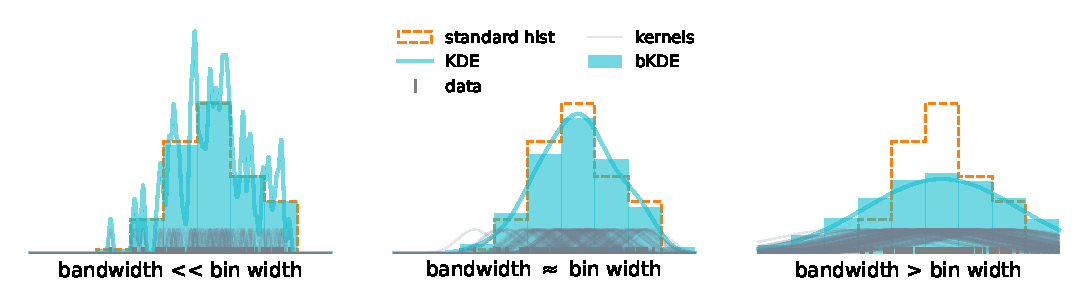
\includegraphics[width=1\textwidth]{relaxed_hist}
    \caption[]{Dependence of the histogram approximation with normal distributions of different standard deviations called bandwidth in the context of \ac{kde}. Depicted in grey small bars on the x-axis are the data points and in grey above them their kernel estimates. Further shown is the standard histogram binned from data, the \ac{kde} and the \ac{bkde} as a histogram calculated from the area under the \ac{kde} for some binning. Adopted from \citep{Simpson_2023}.}
    \label{fig:relaxed_hist}
\end{figure}



\section{Implementation}
Tracing differentiation through software is achievable by recognizing that any software essentially comprises a series of elementary arithmetic operations. Since the analytic solutions for these operations are known, the task reduces to concatenating all these operations and differentiating the resulting function. This is also known as \textit{Automatic Differentiation} and is achieved here with the help of the software package \textsc{jax} \citep{jax2018github} which has several software packages build on top used here. The gradients are processed with \textsc{Optaxsolver} optimizer \citep{jaxopt_implicit_diff} which allows to define a custom loss function and implements a stochastic gradient descent using the Adam optimizer. Integration of the \ac{nn} is accomplished via the machine learning \ac{ml} library \textsc{equinox} \citep{kidger2021equinox}.

While the concept may appear straightforward, one of the challenges that previously hindered its implementation is the difficulty of differentiating across multiple individual software frameworks used in the individual steps of figure \ref{fig:neos}. That this became feasible within a reasonable time frame builds greatly on some transition efforts to the \textsc{Python} programming language from C++ \textsc{root}-based software \citep{ANTCHEVA20092499} used in \ac{hep}. While \textsc{root} was indispensable at its time of emergence, Python offers significant advantages with its ease of use and extensive libraries and frameworks that work seamlessly together, which is essential for the required \ac{ml} techniques. Having all the steps in figure \ref{fig:neos} available as Python packages, has enabled the use of packages like \textsc{jax}, which are not originally connected to \ac{hep}.

The original proposers \citet{Simpson_2023} of \ac{neos} developed differentiable versions of common \ac{hep} tasks, such as hypothesis testing, histogramming, and cut optimization, within a package called \textsc{relaxed} \citep{Simpson_relaxed_version_0_3_0_2023}. Currently, the implementation can only handle the \textsc{HistoSys} modifier described in section \ref{sec:modifiers}, which is standard for managing $\pm1\sigma$ shape uncertainties. However, relevent uncertainties, like normlization uncertainties can be converted into this modification scheme. They successfully tested the pipeline using a toy model \citep{Simpson_neos_version_0_2_0_2021}.

For this thesis, these efforts were further developed within a framework called \textit{\acf{tomatos}} \citep{tomatos} and applied to an \ac{atlas} analysis. This included code refactoring, bug fixing, implementation of weighted histogramming, and building an entire \ac{ml} framework around it. The \ac{ml} framework encompasses data preprocessing, extending compatibility to more than one uncertainty, integration of an appropriate \ac{ml} library, and includes plotting and validation methods. Despite appearing standard, tasks entering the optimization must be implemented in a \textsc{jax}-compatible differentiable manner, which usually requires careful consideration.


\section{Training}\label{sec:neos_training}
In order to build the statistical model each histogram entering it needs to be filled from data during the training. This requires a full dataset of input variables per sample (signal, background estimate, systematic) being processed through the whole pipeline as of figure \ref{fig:neos}. The nominal signal sample for training is the $\ktwov=0$ signal sample, used as a representative for non-\ac{sm} \ktwov hyptheses. The \ac{tomatos} \citep{tomatos} training framework encapsulates the following techniques.

\acp{nn} tend to learn from more frequently observed data. Thus to make use of all available data and to avoid a training class imbalance each sample is upscaled by replicating values to the sample with the largest event content in this case the nominal $\ktwov=0$ signal sample. Since this artificially alters the event counts in the histograms, a scale factor of $n_\text{sample}/n_\text{max}$ is applied to the weights.

Table \ref{tab:neos-samples} gives an overview of used samples and the number of unscaled events they contain. Only uncertainties with a significant impact on an \mhh{} maximum likelihood fit as of figure \ref{fig:m_hh_full_sys_ranking} are used to speed up the training process. These uncertainties are detailed in chapter \ref{sec:systematics} and comprise the 4 $b$-quark branching ratio normalization, the statistical error on the ABCD method transfer factor extraction and the shape uncertainty associated to this method, the four estimated $p_T$ binned uncertainties of the GN2X tagger, the envelope of the scale variations, the statistical errors on the \ktwov signal sample and the background estimate. Table \ref{tab:neos-samples} also reveals that the background estimate is upscaled by a factor of $\sim 2$. 

Input variables per sample are shown in figure \ref{fig:tomatos_inputs_0} and \ref{fig:tomatos_inputs_1}. To ensure a fair training across features and prevent those with large values from dominating the learning process, a min-max scaling is applied to the inputs, transforming the input values to a range between 0 and 1 per feature:
\begin{equation}
    x'=\frac{x - \text{min}(x)}{\text{max}(x)-\text{min}(x)}.
\end{equation}


The optimal model is selected using a validation dataset, which is not used in the training process. The model with the lowest loss on the validation set is chosen. To further verify the validity of this selection, the model's performance is evaluated on a separate test dataset, which is also excluded from the training process. The dataset is divided such that 80\% (34,793 events) is used for training, and 10\% (4,350 events) is used for both validation and testing. After this splitting, the weights each dataset are reweighted to match the event counts of the original dataset before splitting. For example, the training set is reweighted by multiplying by a factor of $1/0.8 = 1.25$.

In addition four samples are processed through the pipeline to estimate the background with the ABCD method described in \ref{sec:abcd}. The transfer factor and its uncertainty is estimated from the \ac{cr} and a shape uncertainty is estimated in the \ac{vr} as described in \ref{sec:bkg_uncertainties}. Per training epoch, which corresponds to a full processing of the dataset, data are reshuffled.

The optimization also optimizes cuts on the invariant mass $m_{jj}$ and the pseudorapidity difference $|\Delta\eta(j,j)|$ of the two \ac{vbf} jets as mentioned in \ref{sec:hh4b_analysis_strategy}. Mathematically, applying a cut can be represented by multiplying the value to be cut with a Heaviside function shifted by the cut value. For a differentiable approximation, a sigmoid function as shown in \ref{fig:activation_fun}(b) is used, which is then multiplied to an event's weight. Statistical uncertainties are included in addition to maintain a natural limit on event counts per bin.

\begin{table}[]
    \centering
    \caption{Samples and available number of unscaled events after the selection described in section \ref{sec:hh4b_analysis_strategy} used in the training. Systematics are described in \ref{sec:systematics}.}
    \begin{tabular}{lr}
        \hline
        Sample (Systematic)                                                      & Events \\ \hline \hline
        Run 2 Data Background Estimate (\ac{sr}, GN2X tags: 1)                   & 21913  \\ \hline
        Signal $\kappa_\mathrm{2V}=0$ (Nominal)                                  & 43492  \\
        Signal $\kappa_\mathrm{2V}=0$ (GN2X pt bin 0 up)                         & 43492  \\
        Signal $\kappa_\mathrm{2V}=0$ (GN2X pt bin 0 down)                       & 43492  \\
        Signal $\kappa_\mathrm{2V}=0$ (GN2X pt bin 1 up)                         & 43492  \\
        Signal $\kappa_\mathrm{2V}=0$ (GN2X pt bin 1 down)                       & 43492  \\
        Signal $\kappa_\mathrm{2V}=0$ (GN2X pt bin 2 up)                         & 43492  \\
        Signal $\kappa_\mathrm{2V}=0$ (GN2X pt bin 2 down)                       & 43492  \\
        Signal $\kappa_\mathrm{2V}=0$ (GN2X pt bin 3 up)                         & 43492  \\
        Signal $\kappa_\mathrm{2V}=0$ (GN2X pt bin 3 down)                       & 43492  \\
        Signal $\kappa_\mathrm{2V}=0$ (Scale Variation $\mu_R = 0.5, \mu_F=0.5)$ & 43492  \\
        Signal $\kappa_\mathrm{2V}=0$ (Scale Variation $\mu_R = 0.5, \mu_F=1.0)$ & 43492  \\
        Signal $\kappa_\mathrm{2V}=0$ (Scale Variation $\mu_R = 1.0, \mu_F=0.5)$ & 43492  \\
        Signal $\kappa_\mathrm{2V}=0$ (Scale Variation $\mu_R = 1.0, \mu_F=1.0)$ & 43492  \\
        Signal $\kappa_\mathrm{2V}=0$ (Scale Variation $\mu_R = 1.0, \mu_F=2.0)$ & 43492  \\
        Signal $\kappa_\mathrm{2V}=0$ (Scale Variation $\mu_R = 2.0, \mu_F=1.0)$ & 43492  \\
        Signal $\kappa_\mathrm{2V}=0$ (Scale Variation $\mu_R = 2.0, \mu_F=2.0$) & 43492  \\ \hline
        Run 2 Data (\ac{cr}, GN2X tags: 1)                                       & 142443 \\
        Run 2 Data (\ac{cr}, GN2X tags: 2)                                       & 544    \\
        Run 2 Data (\ac{vr}, GN2X tags: 1)                                       & 57098  \\
        Run 2 Data (\ac{vr}, GN2X tags: 2)                                       & 243    \\
    \end{tabular}
    \label{tab:neos-samples}
\end{table}


\begin{figure}
    \centering
    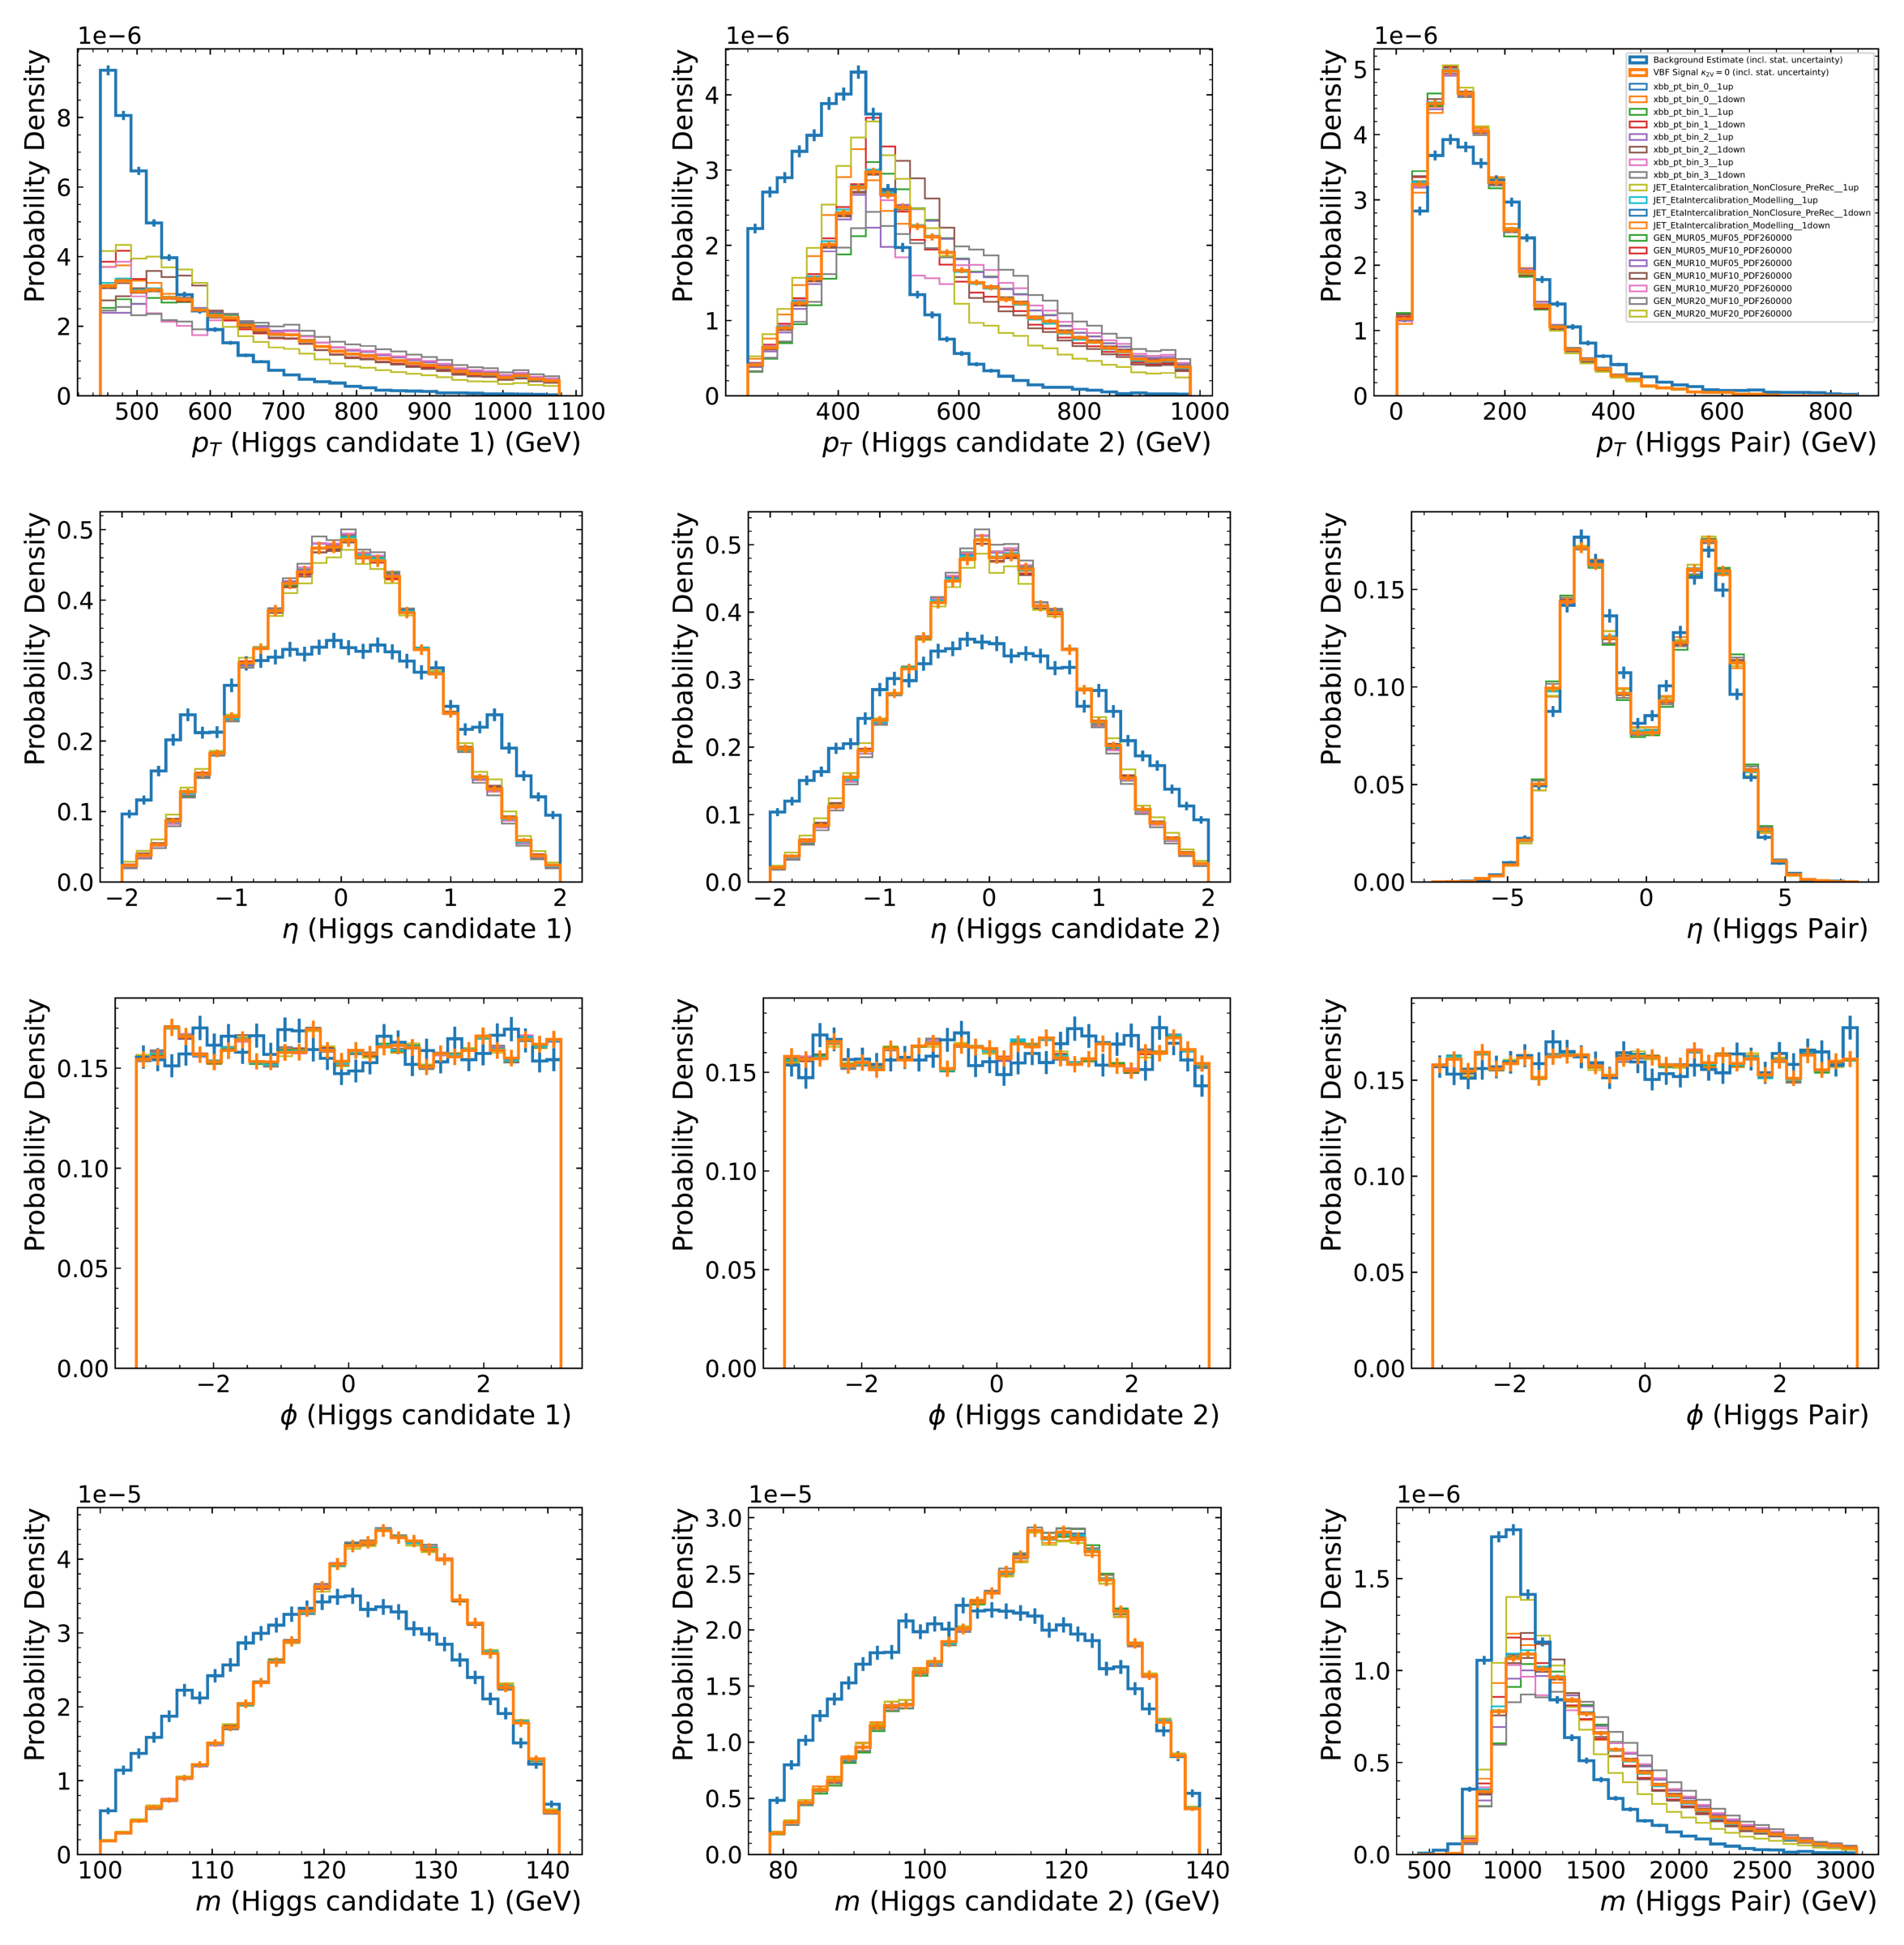
\includegraphics[width=1\textwidth]{neos_results/tomatos_inputs_0}
    \caption[]{Neos input variables (1/2): The coloums from left to right correspond to the four vectors of the leading Higgs candidate, the subleading Higgs candidate and the Higgs Pair system. A legend valid for all figures is shown in the upper right figure.}
    \label{fig:tomatos_inputs_0}
\end{figure}



\begin{figure}
    \centering
    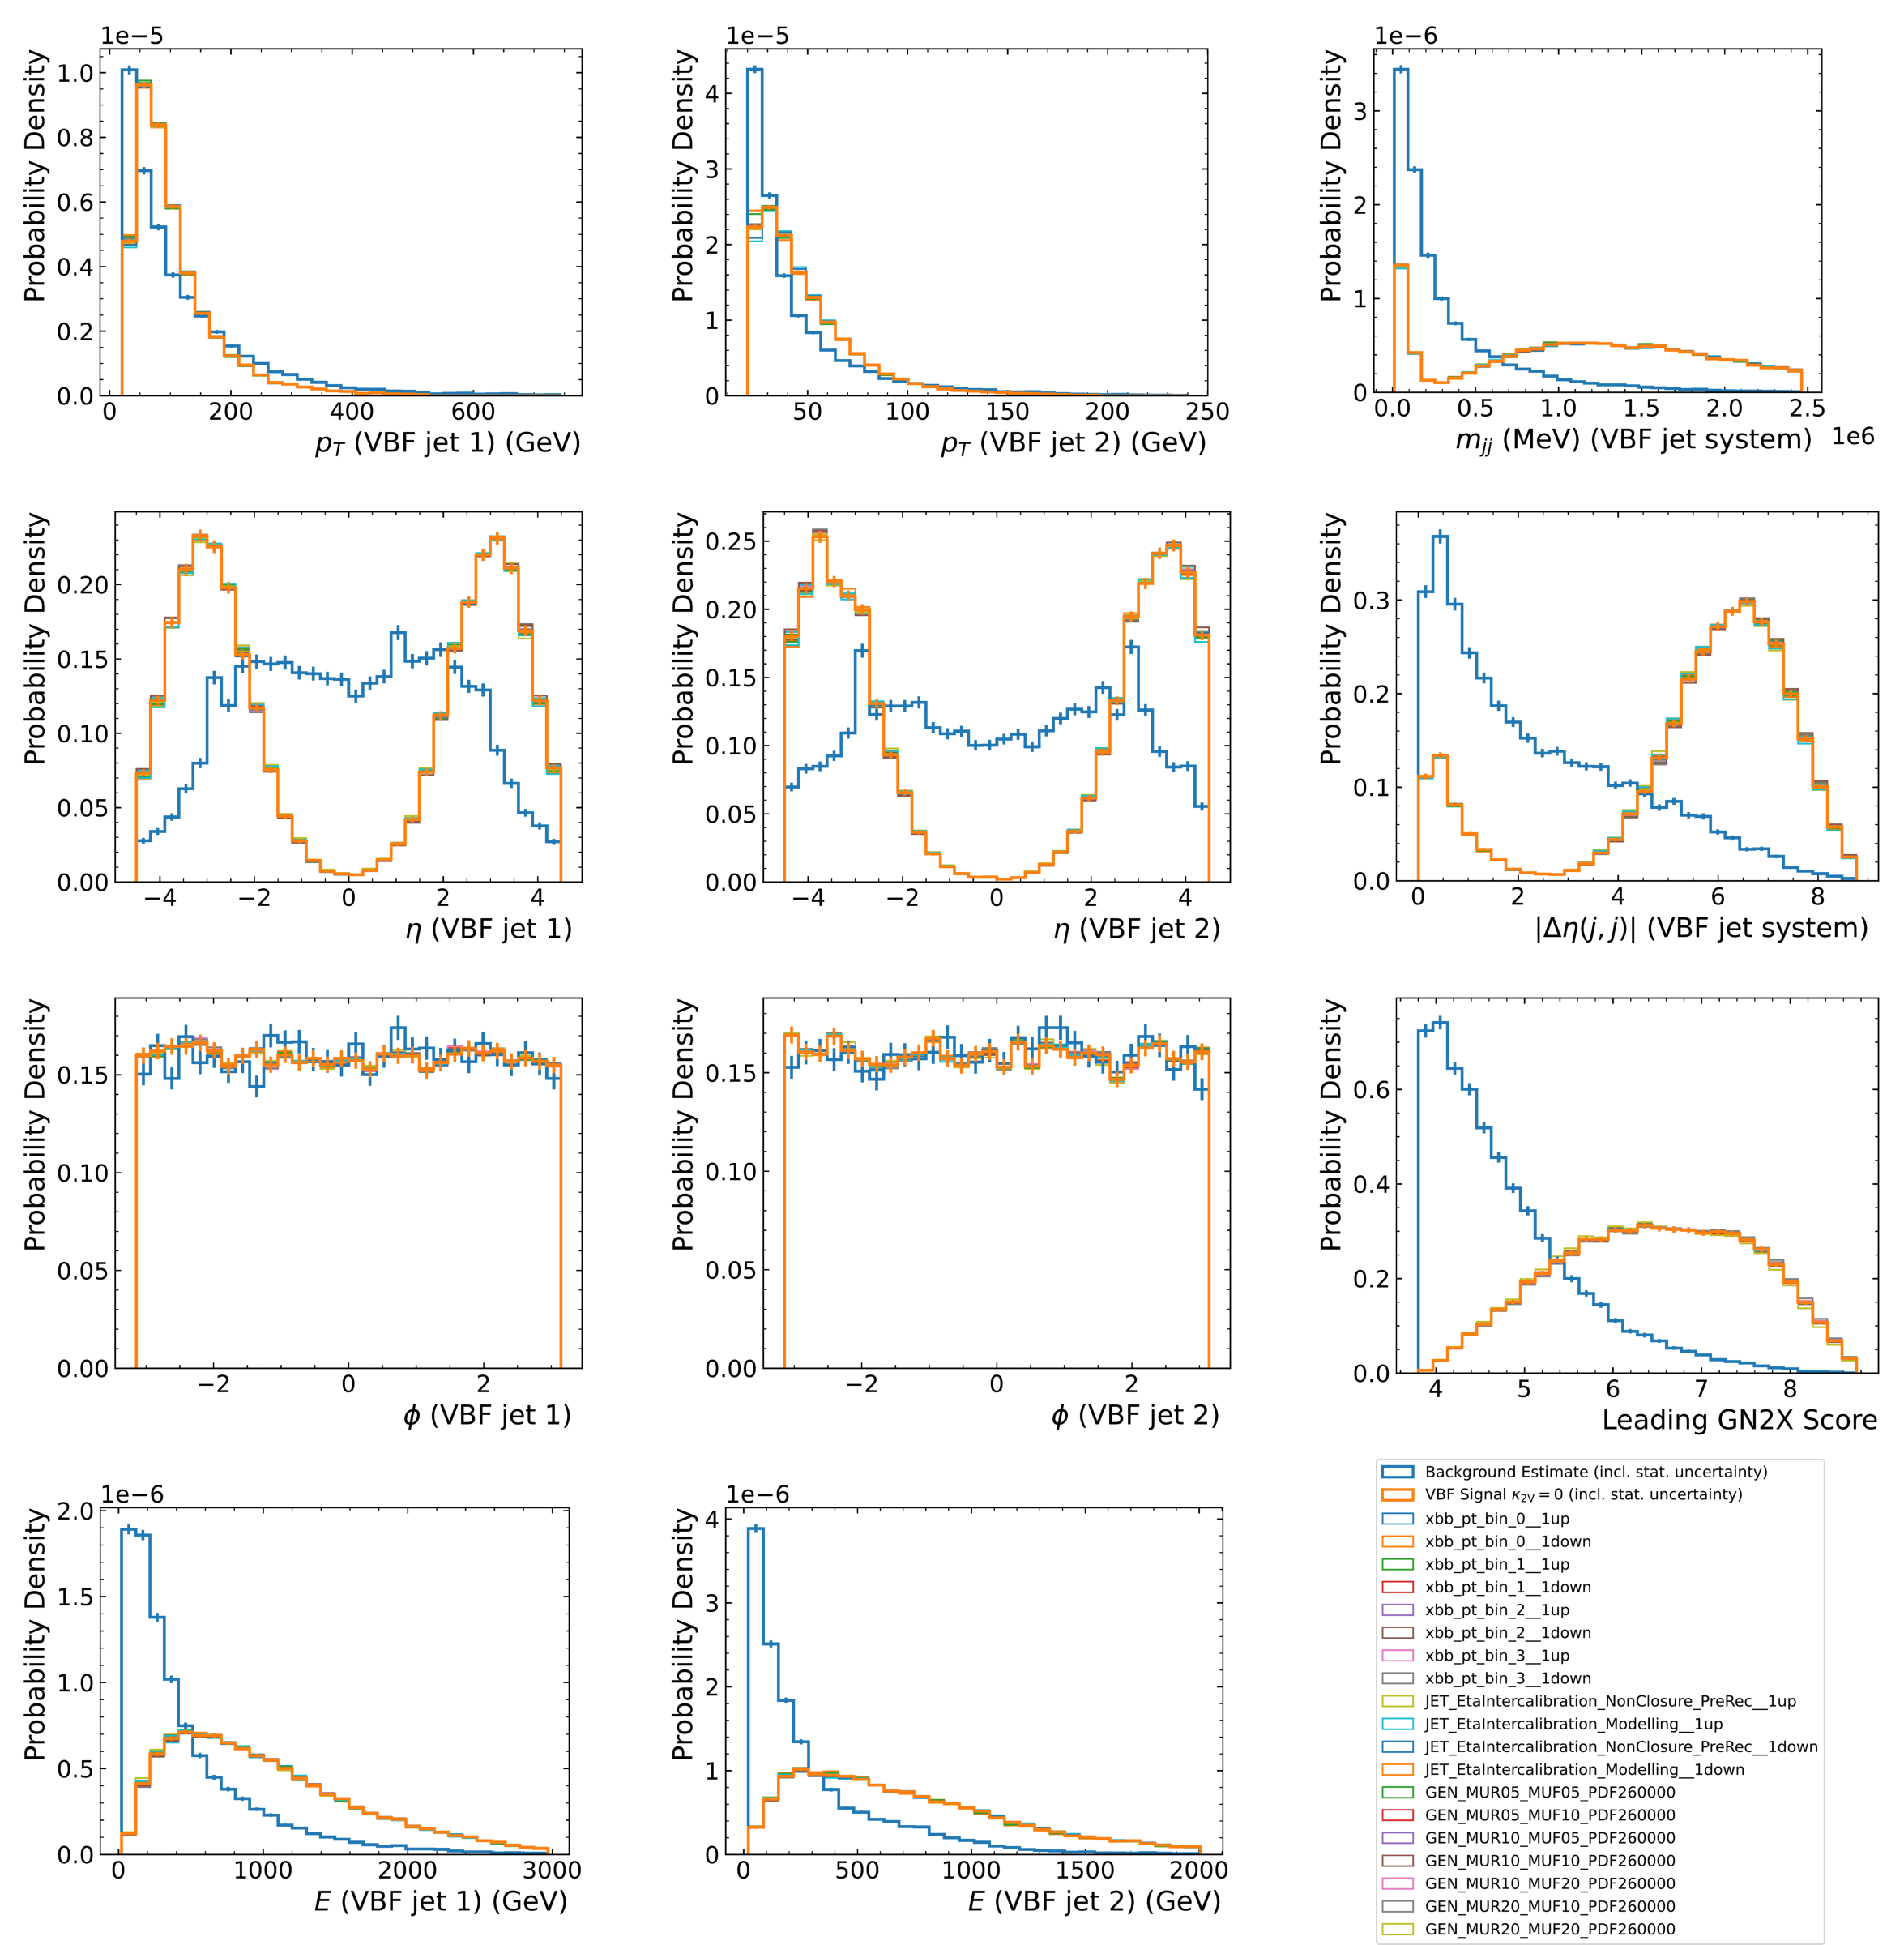
\includegraphics[width=1\textwidth]{neos_results/tomatos_inputs_1}
    \caption[]{Neos input variables (2/2): Columns from left to right: Four vectors of the two vbf jets and the leading GN2X score in the event is depicted above the legend.}
    \label{fig:tomatos_inputs_1}
\end{figure}
